\begin{center}
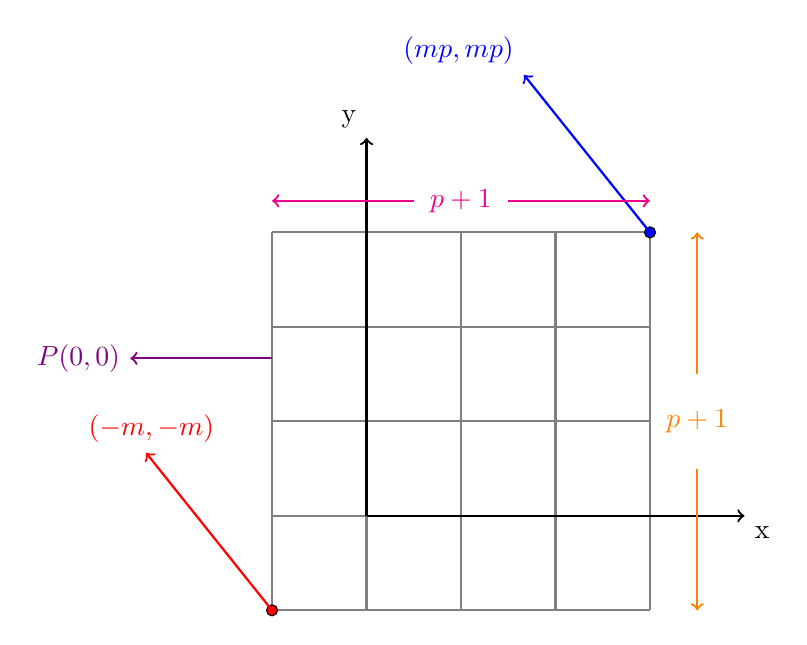
\begin{tikzpicture}[scale=0.4]

    %\fill[gray!30] (0,0) rectangle (12,12);

   

    % Second Grid (dashed), positioned 2 units left and 3 units below
   
    % \draw[step=3cm,black,dashed, thick] (0,0) grid (12,12);
    % \filldraw[fill=blue] circle (5pt) ;
    % \draw[orange, <->, thick] (-0.2, 0) -- (-1.5, 0) node[below] {\textbf{a}};
    % \draw[magenta, <->, thick] (0, -0.2) -- (0, -2.5) node[right] {\textbf{b}};
    % \draw[blue, ->, thick] (0, 0) -- (-4, 5) node[anchor=south east] {\textbf{ $(-m+a,-m+b)$}};

    
    

    %\begin{scope}[xshift=-1.5cm, yshift=-2.5cm]
        \draw[step=3cm,gray, thick] (0,0) grid (12,12);
        \filldraw[fill=red] circle (5pt) ;
        \filldraw[fill=blue](12,12) circle (5pt) ;
        \draw[red, ->, thick] (0, 0) -- (-4, 5) node[above] {\textbf{ $(-m,-m)$}};
        \draw[thick,->,black] (3,3) -- (15,3) node[anchor=north west] {x};
        \draw[thick,->,black] (3,3) -- (3,15) node[anchor=south east] {y};

        \draw[blue, ->, thick] (12, 12) -- (8, 17) node[anchor=south east] {\textbf{ $(mp,mp)$}};
        
    %\end{scope}

    %\draw[thick,->,violet] (0,11) -- (-7,11) node[left] {$P(a,b)$};
    \draw[thick,->,violet] (0,8) -- (-4.5,8) node[left] {$P(0,0)$};
    \draw[thick,->,magenta] (4.5,13) -- (0,13);
    \node[magenta] at (6,13) {$p+1$};
    \draw[thick,->,magenta] (7.5,13) -- (12,13);

    \draw[thick,->,orange] (13.5,4.5) -- (13.5,0);
    \node[orange] at (13.5,6) {$p+1$};
    \draw[thick,->,orange] (13.5, 7.5) -- (13.5,12);

    

\end{tikzpicture}
\end{center}